V této podkapitole se pustím do samotného testování JPA (ORM) frameworků. Mezi testované JPA implementace jsem zařadil (Hibernate, EclipseLink,OpenJPA, DataNucleus a BatooJPA).
Veškeré výsledky jsou opět v milisekundách.

\begin{figure}[!h]
\begin{subfigure}[b]{1\textwidth}
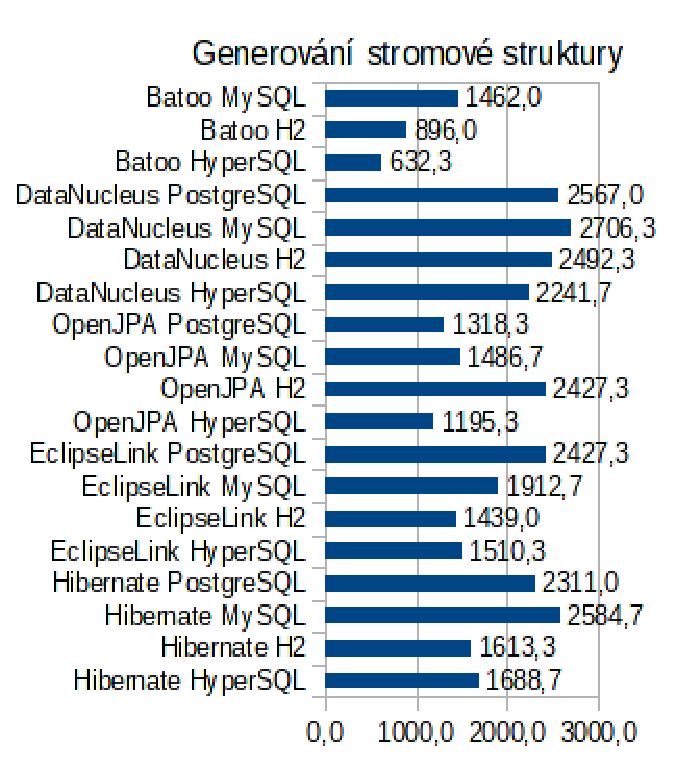
\includegraphics[width=25em]{obr/bench/jpa1}
\end{subfigure}
\begin{subfigure}[b]{1\textwidth}
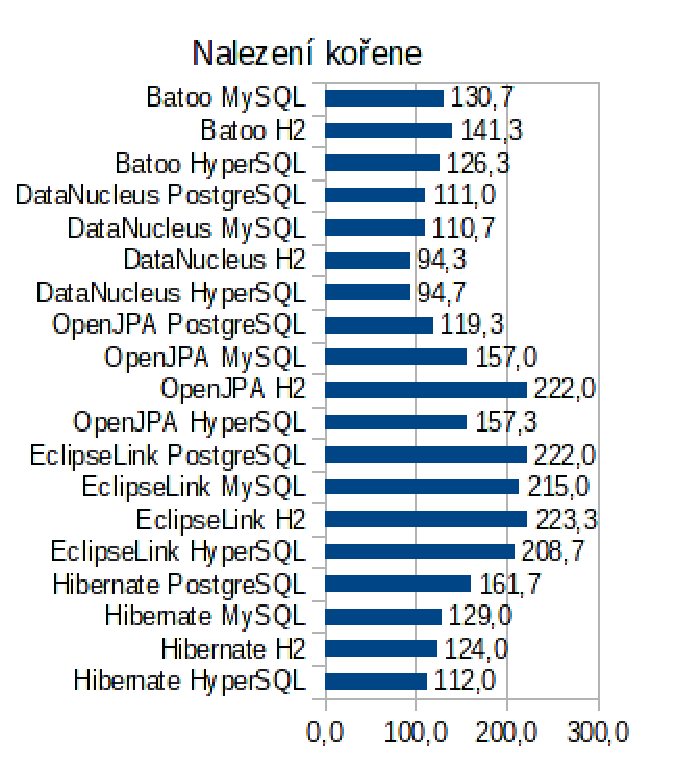
\includegraphics[width=25em]{obr/bench/jpa2}
\end{subfigure}
\end{figure}

\begin{figure}
\begin{subfigure}[b]{1\textwidth}
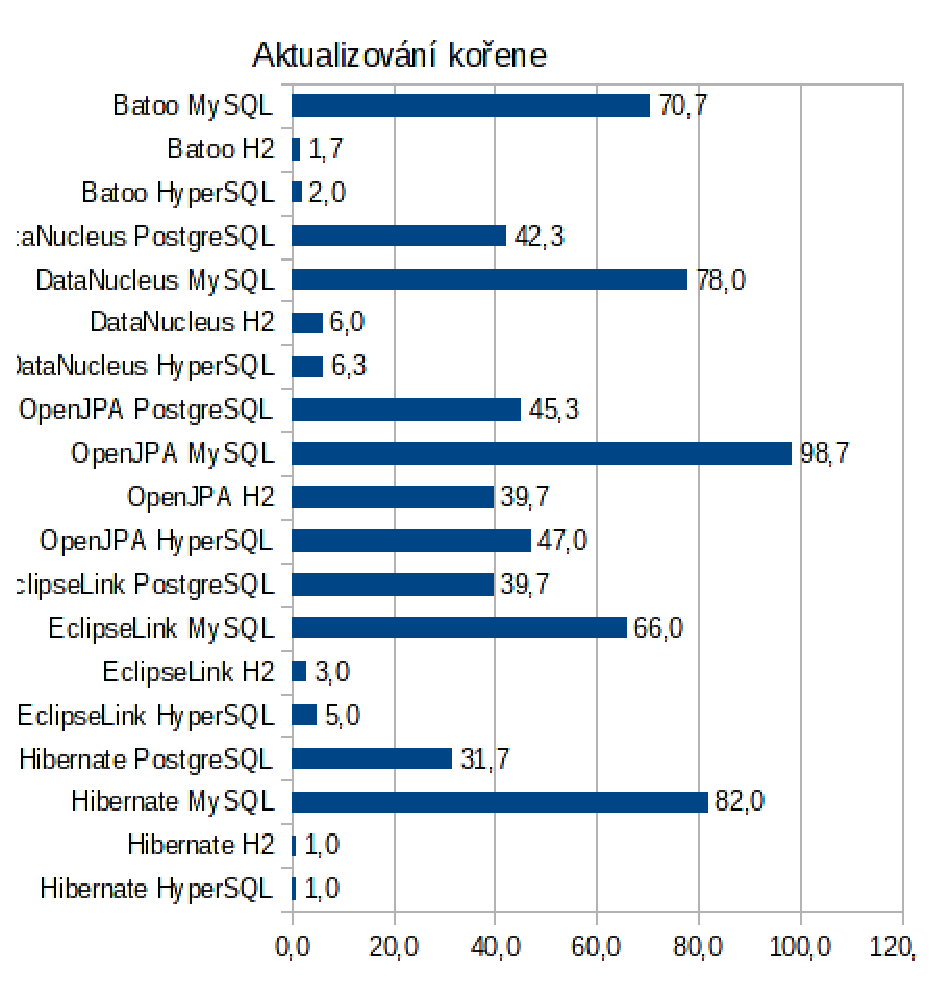
\includegraphics[width=25em]{obr/bench/jpa3}
\end{subfigure}
\begin{subfigure}[b]{1\textwidth}
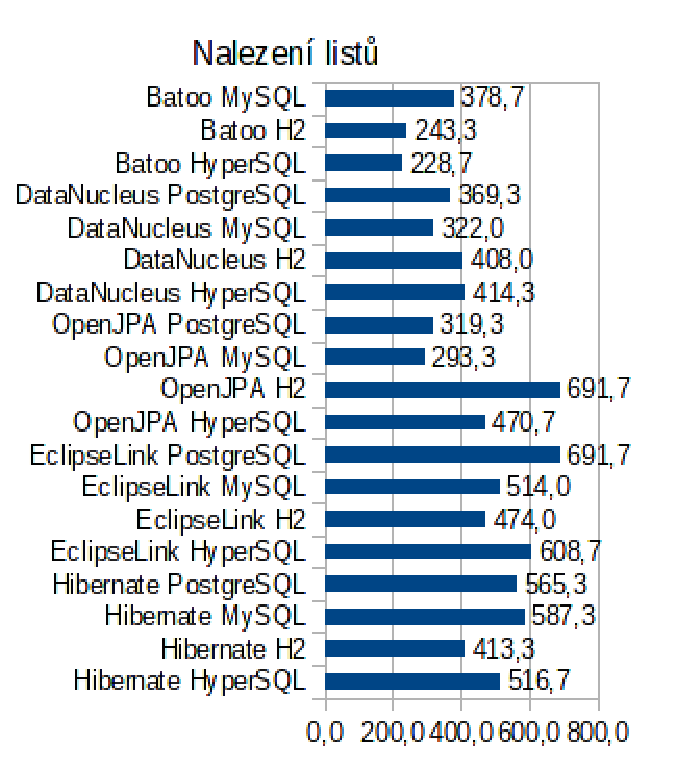
\includegraphics[width=25em]{obr/bench/jpa4}
\end{subfigure}
\end{figure}


\begin{figure}[!h]
\begin{subfigure}[b]{1\textwidth}
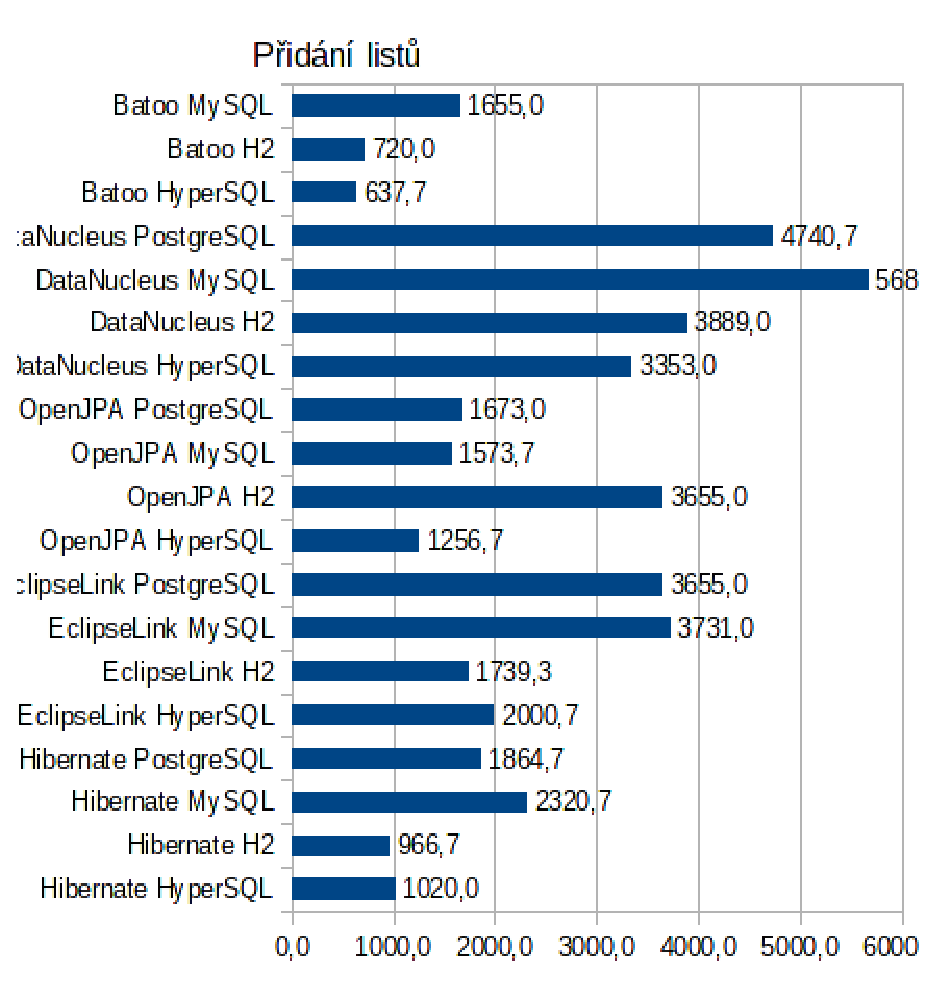
\includegraphics[width=25em]{obr/bench/jpa5}
\end{subfigure}
\begin{subfigure}[b]{1\textwidth}
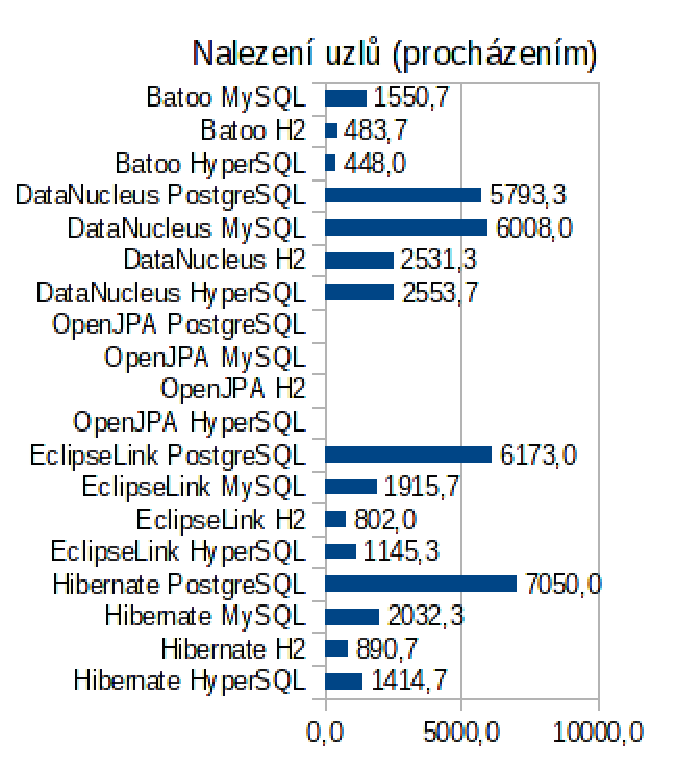
\includegraphics[width=25em]{obr/bench/jpa6}
\end{subfigure}
\end{figure}

\begin{figure}
\begin{subfigure}[b]{1\textwidth}
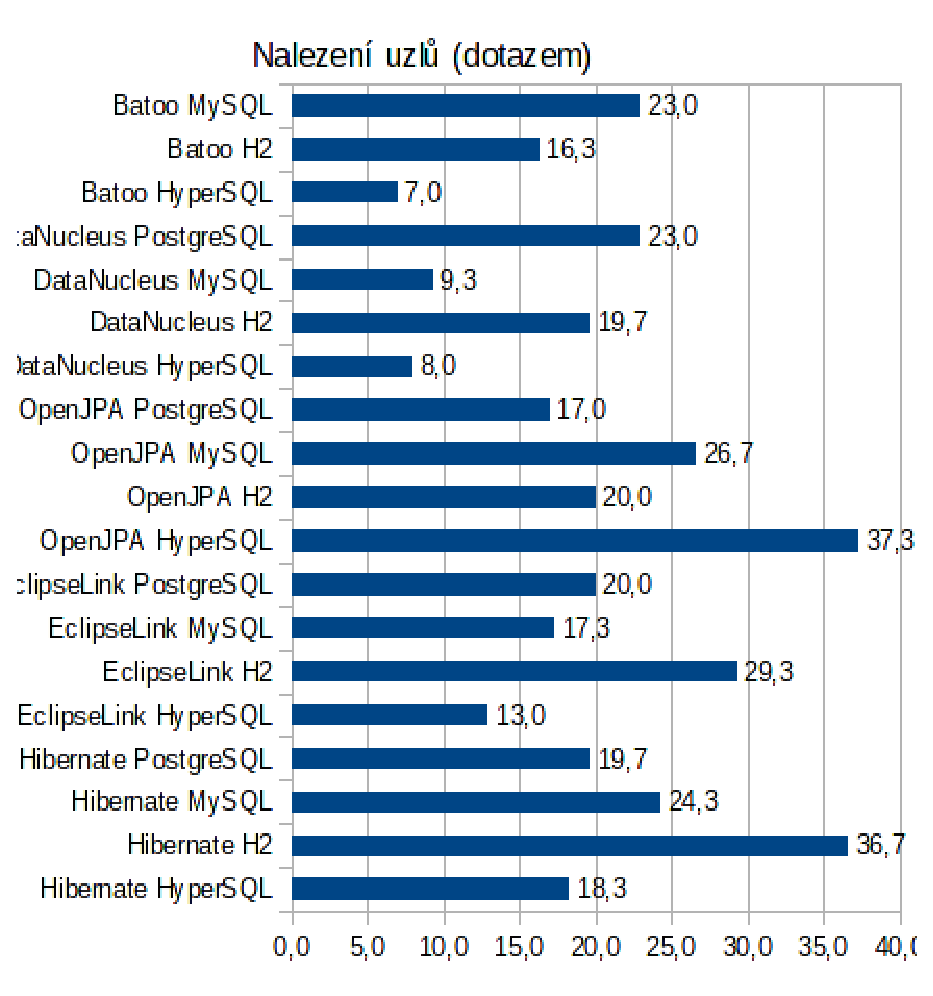
\includegraphics[width=25em]{obr/bench/jpa7}
\end{subfigure}
\begin{subfigure}[b]{1\textwidth}
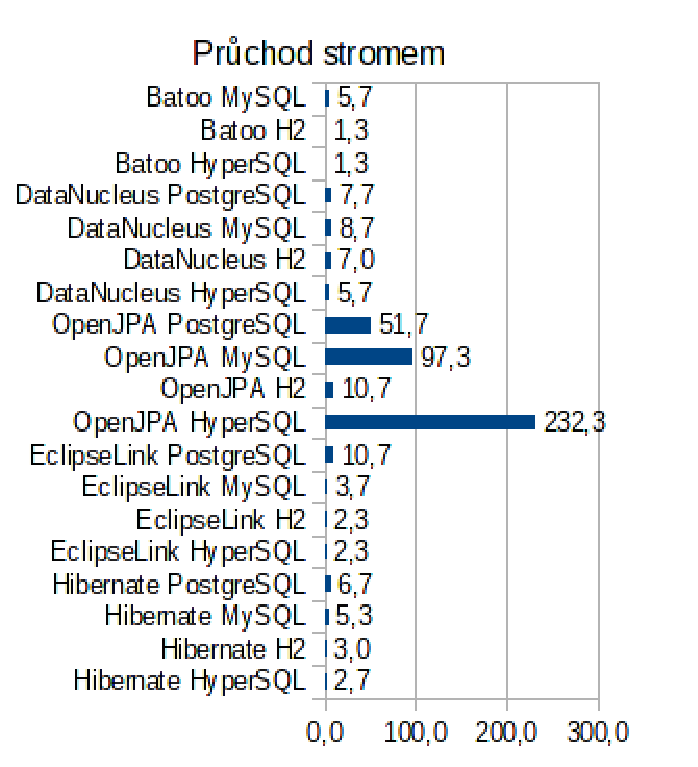
\includegraphics[width=25em]{obr/bench/jpa8}
\end{subfigure}
\end{figure}

\begin{figure}[!h]
\begin{subfigure}[b]{1\textwidth}
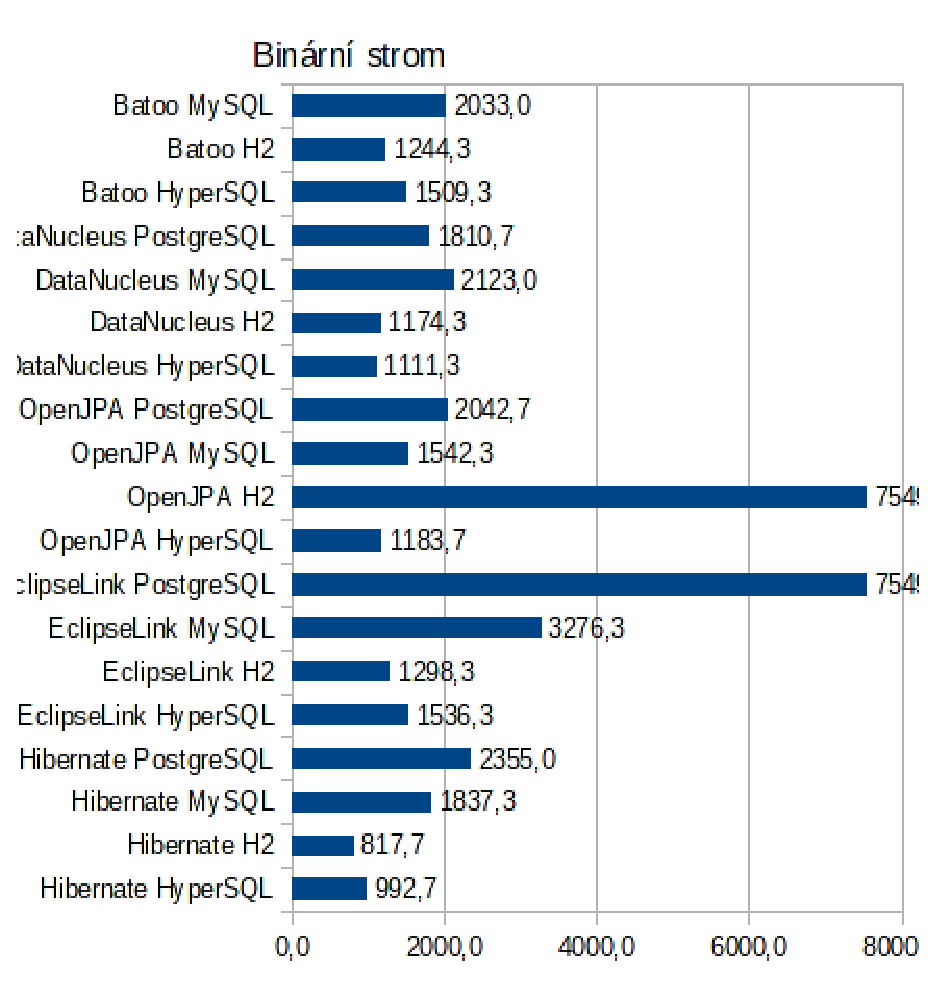
\includegraphics[width=25em]{obr/bench/jpa9}
\end{subfigure}
\begin{subfigure}[b]{1\textwidth}
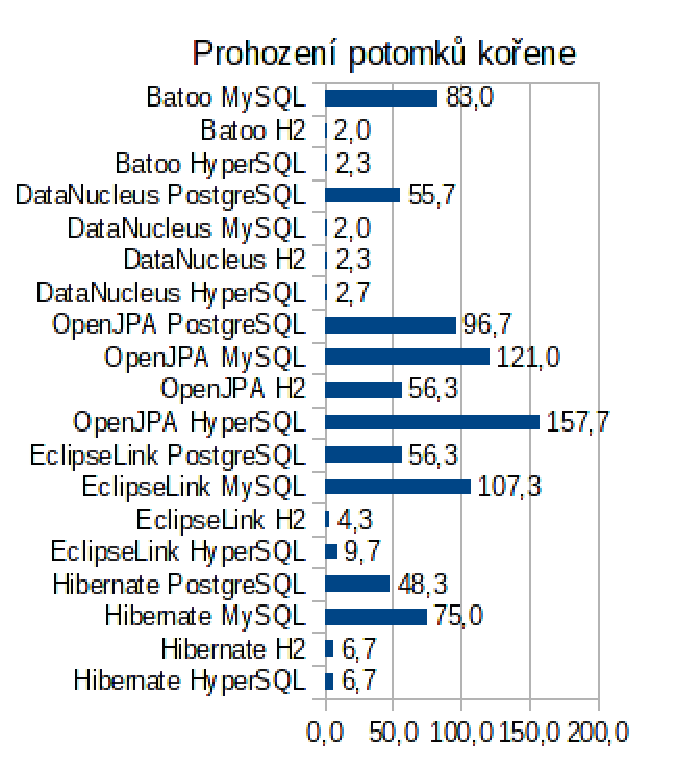
\includegraphics[width=25em]{obr/bench/jpa10}
\end{subfigure}
\end{figure}

\begin{figure}
\begin{subfigure}[b]{1\textwidth}
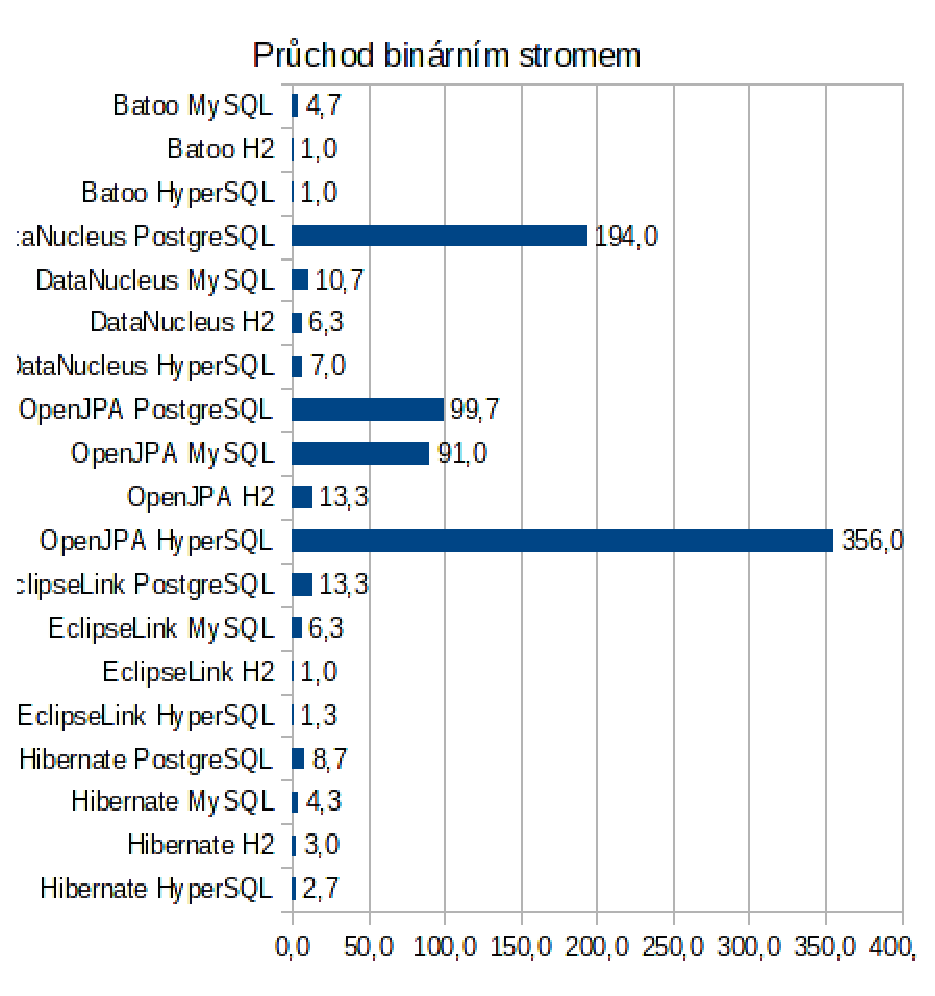
\includegraphics[width=25em]{obr/bench/jpa11}
\end{subfigure}
\begin{subfigure}[b]{1\textwidth}
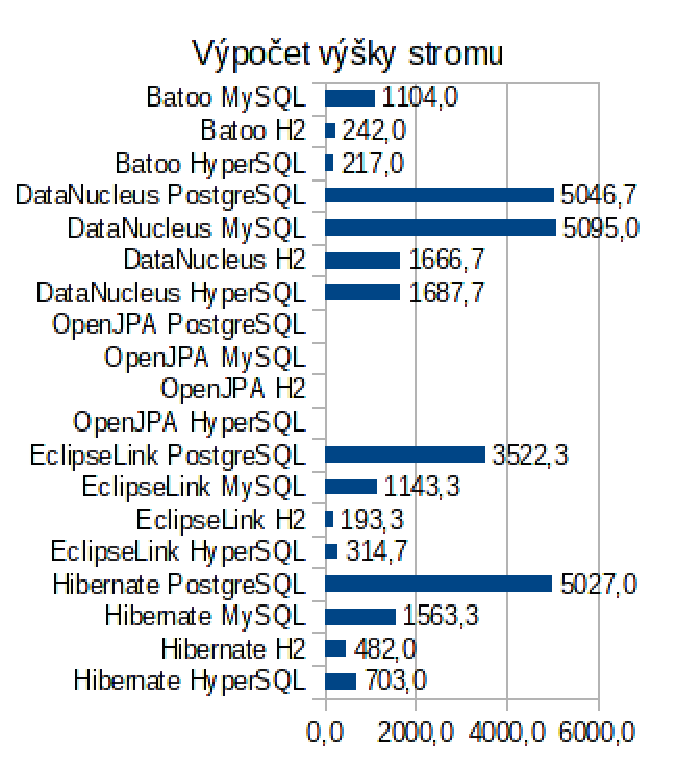
\includegraphics[width=25em]{obr/bench/jpa12}
\end{subfigure}
\end{figure}

\begin{figure}[!h]
\begin{subfigure}[b]{1\textwidth}
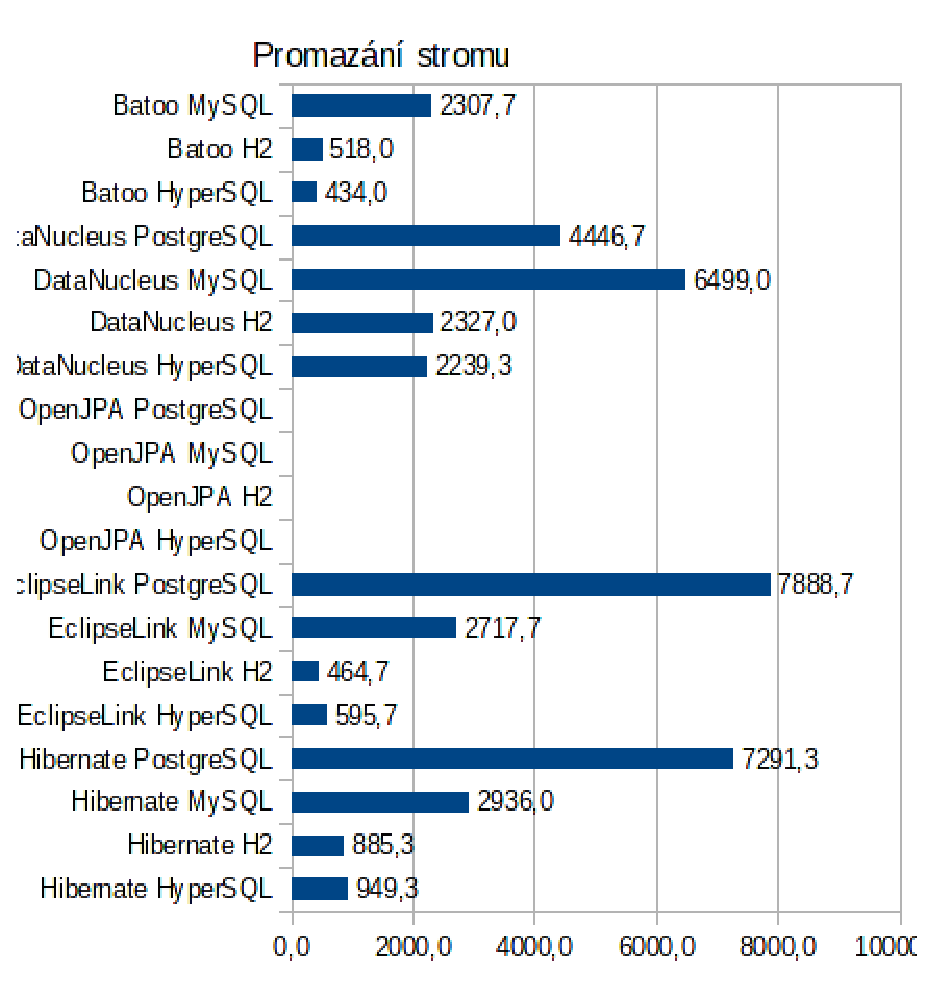
\includegraphics[width=25em]{obr/bench/jpa13}
\end{subfigure}
\begin{subfigure}[b]{1\textwidth}
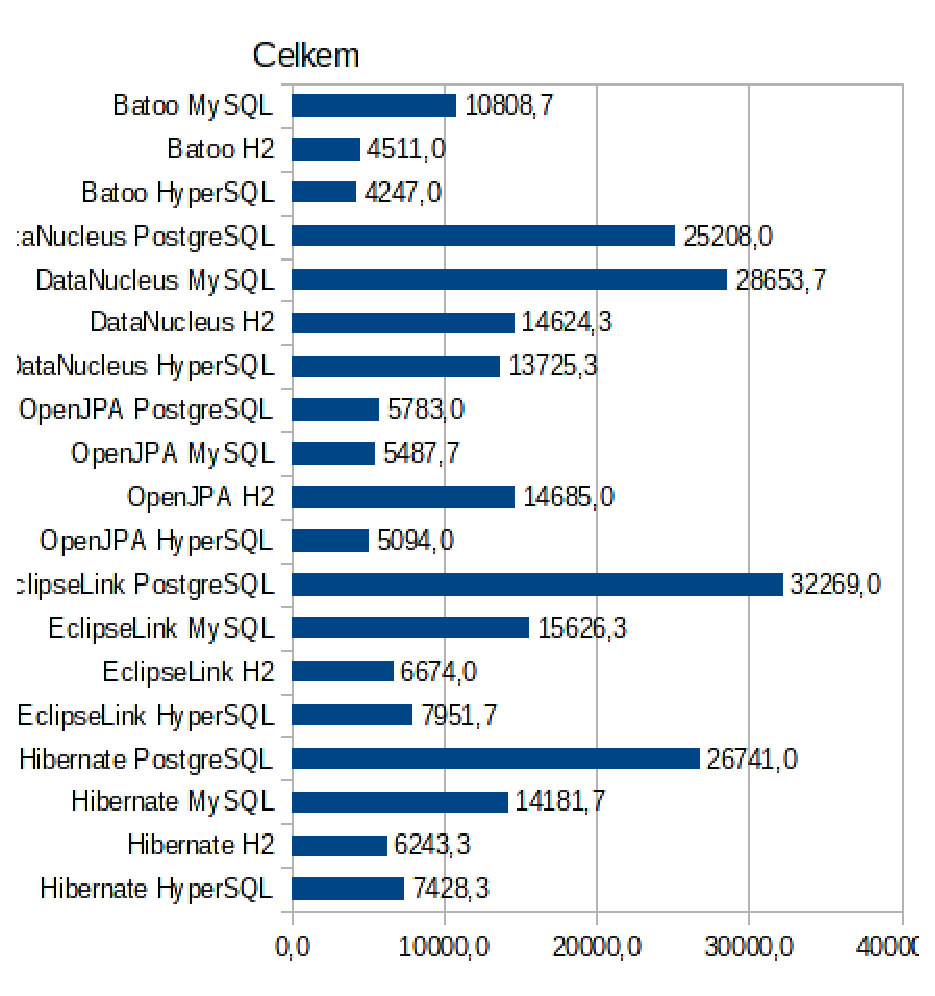
\includegraphics[width=25em]{obr/bench/jpa14}
\end{subfigure}
\end{figure}
